\documentclass[a4paper,10pt]{article}
\usepackage[margin=2.5cm]{geometry}
\usepackage[utf8]{inputenc}
\usepackage[colorlinks=true,urlcolor=blue]{hyperref}
\usepackage{amsmath}
\usepackage{graphicx}
\usepackage{float}
\usepackage{caption}
\usepackage{subcaption}

%\usepackage{listings} %Alternative to minted
\usepackage{minted}



\setlength{\parindent}{0em}
\setlength{\parskip}{1em}

\begin{document}
\begin{titlepage}
    \centering
    \vspace*{2cm}
    {\Huge \textbf{1RT730 Project Report} \par}
    \vspace{0.5cm}
    {\LARGE Harald - The Ultimate Swedish Chatbot \par}
    
    \vspace{2cm}
    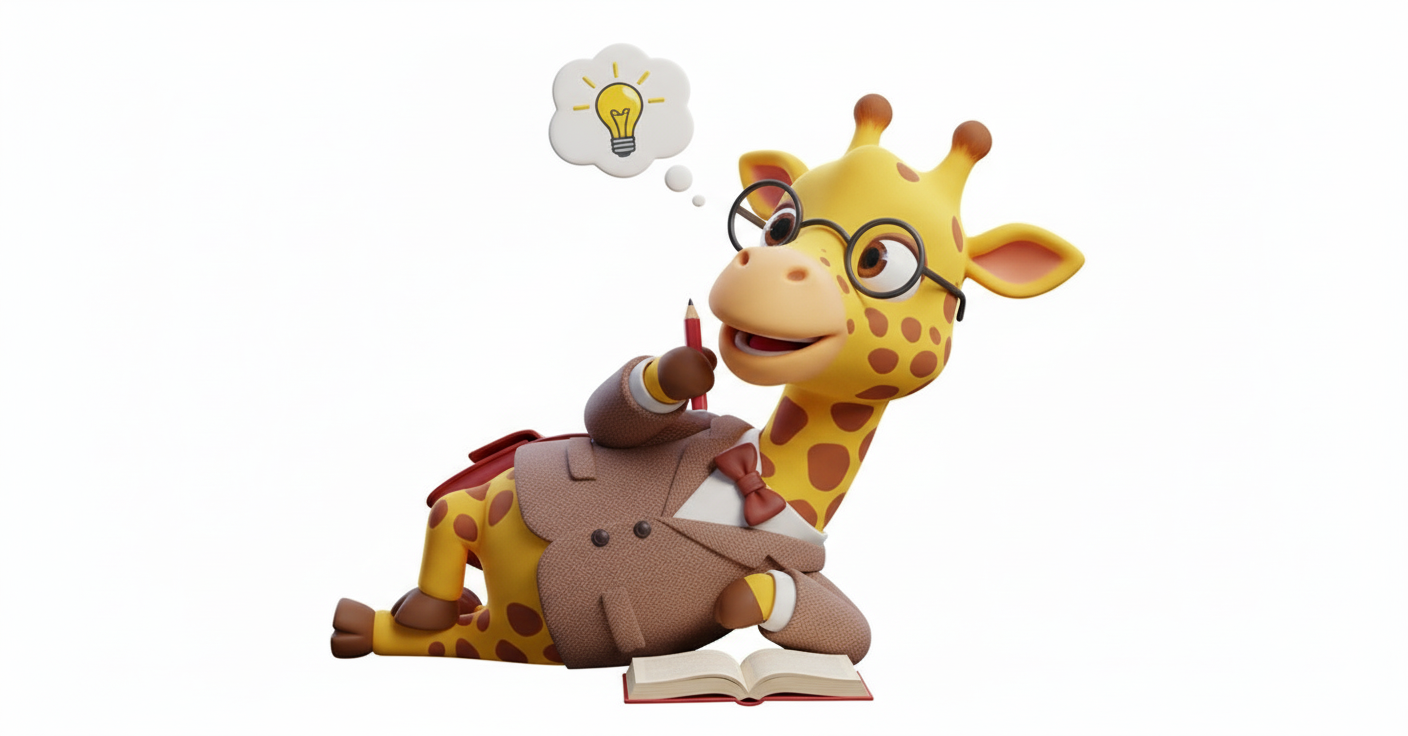
\includegraphics[width=0.6\textwidth]{cute_thinking_harald.png} % your image
    \vspace{2cm}
    
    {\Large Joel Sundin, Petter Möllerström, Rahul Sebastian Peter \par}
    \vspace{1cm}
    {\large \today \par}
\end{titlepage}   
\newpage

 \section{Introduction}
Learning Swedish as a non-native speaker presents significant challenges, particularly when opportunities for interactive practice and real-time feedback are limited. To address these challenges, this work proposes \textit{Harald}, an AI-driven language learning application that leverages Large Language Models (LLMs), quizzes, and flashcard functionalities to enhance engagement and personalization in language acquisition.

Harald integrates multiple learning modalities to support comprehension, vocabulary retention, and conversational skills. Beyond individual learning, Harald contributes to societal language inclusivity by supporting immigrants, students, and professionals in their integration into Swedish society. The primary contribution of this study lies in the integration of LLM-based interaction within a structured learning framework, enabling personalized practice, targeted feedback, and contextual understanding in a scalable and accessible manner.

Harald is implemented as a web-based application, allowing learners to access its features directly through a standard browser without the need for local installation. This design choice enhances accessibility and convenience, enabling learners to practice Swedish anytime and anywhere, whether on desktop or mobile devices. By combining cloud-based LLM computation with an intuitive browser interface, Harald ensures that advanced language processing capabilities are delivered seamlessly to users, while maintaining a lightweight and user-friendly experience.

The system’s web-based nature also facilitates easy updates and integration of new exercises or models, ensuring that learners always benefit from the latest improvements in AI-driven language education. Overall, Harald provides a comprehensive, adaptive, and accessible environment for Swedish language learning, bridging the gap between traditional pedagogical methods and modern AI-assisted instruction.


\section{Dataset}
In this section, describe the dataset(s) that support your LLM application. Specify their source, size, and type (e.g., text, images, multimodal data). Discuss any preprocessing or data-cleaning steps applied, aand methods used to prepare the data for training, fine-tuning, or evaluation. If the application relies on prompt engineering or synthetic data generation instead of a formal dataset, explain the rationale and design choices. Highlight any limitations, biases, or challenges present in the dataset, and justify why it is suitable for your application.

\section{Architecture}
This section should outline the overall design and workflow of the LLM-based application. Present the system architecture, describing how inputs are processed, how the LLM is integrated, and how outputs are generated and refined. If applicable, explain supporting components such as retrieval-augmented generation (RAG) modules, safety filters, knowledge bases, or user interfaces. Visual aids such as figures or flowcharts are encouraged to illustrate the data flow and interactions between components. Also please justify the design choices and explain how the architecture supports the application's goals.

\section{Results}
In this section, present the outcomes of your experiments or evaluations. Provide both quantitative results (e.g., accuracy, precision, recall, BLEU, latency) and qualitative analyses (e.g., case studies, user feedback, example outputs). Where possible, compare the performance of your system against baseline methods or alternative approaches. Discuss the strengths of your application as well as its limitations, including cases where it may fail or underperform. Use tables, graphs, or figures to support clarity and emphasize key findings.

\section{Societal Impact}
Here, reflect on the broader implications of your LLM application for society. Discuss potential benefits such as improved accessibility, efficiency, education, or democratization of knowledge. At the same time, critically examine possible risks, including issues of bias, fairness, privacy, misuse, or environmental impact. Consider ethical challenges and describe mitigation strategies, such as transparency, safety mechanisms, or human oversight. This section should demonstrate awareness of the responsibility associated with deploying LLM-based systems in real-world contexts.

	
\hfill \break
\textit{\textbf{Use of generative AI}}

Write a few sentences if you have or have not used any generative AI, and if so how.


\hfill \break
\textit{\textbf{Note}}

Report should be max. 4-6 pages long.

	
\begin{thebibliography}{1}

	%\bibitem{Item} Add here.
		
\end{thebibliography}

	
	
%	\pagebreak
%	
%	\appendix
%	\section{Code}
%	\label{app:code}
%	
%	\inputminted[frame=lines,framesep=2mm,linenos]{python}{your_code.py}
%	
\end{document}
